\newpage
\chapter{Literature review}
\label{Literature}

\lhead{\emph{Literature Review}} % Set the left side page header to "Symbols"

Though Black's result~\citep{Black_1948} is a famous positive result, it is far from the only positive result relating to domain restrictions. We first look into various domain restrictions and their properties. To fully understand why single peakedness is specifically desirable we outline the political and philosophical reasons first, after which we elaborate on the mechanism through which deliberation should result in single peakedness according to \citet{List_2002}. Finally, for completeness' sake, we mention critiques of this theory.

\section{Domain Restrictions}
A voting domain $\mathcal{D}$ is the domain of all possible voting profiles \(R\) given some number of voters $N$ and some number of alternatives $|X|$. Intuitively, this is simple the space of all possible outcomes of some election. Put more formally, we get.

\begin{definition}{Domain}{domain}
	{
		Given a set of voters $N$, alternatives $A$, and conditions $C$, the domain $\mathcal{D}$ of an election is the set of all profiles $R$ such that all conditions $C$ are satisfied.
	}
\end{definition}

When we consider the domain of an election, one particular profile is the source of many impossibility results in social choice, namely, the Condorcet cycle. To understand why this profile is problematic, let us first define a notion of aggregation, the \textit{majority relation} is the preference relation we get when we compare all alternatives pairwise, and construct a preference profile from this. 

\begin{example}{Majority relations}{maj-rel}
	\begin{minipage}{0.15\linewidth}
		\begin{tabular}{ccc}
			\toprule
			$v_1$ & $v_2$ & $v_3$ \\
			\midrule
			a & b & a \\
			b & c & c \\
			c & a & b \\
			\bottomrule
		\end{tabular}
	\end{minipage}
	\hspace{2em}
	\begin{minipage}{0.70\linewidth}
		Given the profile on the left, we first start by comparing $a$ to $b$, both voters 1 and 3 prefer $a$ to $b$, thus the majority has prefers $a$ to $b$. Comparing $b$ to $c$, we see again that the majority prefers $b$ to $c$. Finally, comparing $a$ to $c$ we see $a$ is again preferred. Thus, the majority relation is $a \prefmaj b \prefmaj c$
	\end{minipage}
\end{example}

One property of the majority relation, that is both desirable, yet violated by the Condorcet cycle is that of transitivity. We define the transitivity on the majority relation as follows

\begin{definition}{Transitivity}{maj-trans}
	A (majority) relation is transitive, if for any triplet $a, b, c \in A$, if $a \prefmaj b$ and $b \prefmaj c$, then $a \prefmaj c$.
\end{definition}

Intuitively it is clear why such a property is desirable, if the majority can agree on the ordering of the alternatives, it must be easier to pick a winner. Unfortunately this is not always the case, with the most famous example being the Condorcet cycle. This is a profile with 3 voters and 3 alternatives, in which all alternatives are ranked in all positions, \cref{tab: Condorcet} show a particular instance of a Condorcet cycle.

 
\begin{table}[h]
\centering
\begin{tabular}{ccc}
	\toprule
	$v_1$ & $v_2$ & $v_3$ \\
	\midrule
	a & b & c \\
	b & c & a \\
	c & a & b \\
	\bottomrule
\end{tabular}
	\caption{The Condorcet cycle, showing all alternatives in each position}
	\label{tab: Condorcet}
\end{table}

% TODO: Find the paper that specifies the number of voters needed for a neutral and annonymous rule to never return a full tie.
Clearly this profile presents problems, as each possible outcome, would also have a majority of voters preferring another. Naturally one might consider if this profile might even come up in practice, since though conceivable it seems generally unlikely that there exists a perfect split in opinions. Quite naturally one of the first ``solutions" one might consider is when the number of voters is not a multiple of the number of alternatives, though this is hardly a solution, if this is the case, it is in fact possible to pick a winner through a simple rule such as the plurality rule [CITATION NEEDED]. This is the first example of a domain restriction, we define it as follows

\begin{definition}{$\domain{No-tie}$}{dom-ties}
	Let $X$ be the set of alternatives and $N$ be the set of voters, of size $n$ such that $n \neq k \cdot |X|$. We call the domain of all outcomes $\domain{No-tie}$.
\end{definition}

This allows us to state our first proposition.

\begin{proposition}
	The plurality rule never returns a $|X|$-way tie between alternatives when applied to $\domain{No-tie}$
\end{proposition}

\begin{proof}
	Assume, for the sake of contradiction, the plurality in fact does return a tie this must mean that all alternatives were ranked first an equal number of times, call this $k$, necessarily then, we have need exactly $k \cdot |X|$ voters, but this leads to a contradiction, as this would no longer be inside $\domain{No-tie}$.
\end{proof}

This is a simple result, but it leads to way to more interesting ones. For this we need to specify more clearly in what ways we can restrict our domains. \citet{Gaertner_2002} establishes 2 ways in which a domain can be restricted. Firstly we can restrict the domain to a number of voters or alternatives, which is what we did in $\domain{No-tie}$. Secondly, the domain can be restricted to have a certain structure, such as being single-peaked. Furthermore, \citet{Elkind_Lackner_Peters_2022} establish the \textit{hereditary}

\begin{definition}{Hereditary \textnormal{(\citet{Elkind_Lackner_Peters_2022})}}{dom-hereditary}
	A domain restriction onto $\domain{ }$ is \textit{hereditary} if, for every profile $P \in \domain{ }$, and every profile $P'$, that can be obtained by deleting voters and alternatives from $P$, $P'$ is also in $\domain{ }$
\end{definition}

\subsection{Condorcet Domain}
If our goal is to prevent Condorcet cycles, or in general have transitive majority relations, the best we could hope to do is to apply our domain restriction such that our domain contains all profiles $P$ such that $P$ has a (weak) Condorcet winner. We call this domain $\domain{Condorcet}$. Under this domain, let $\votingrule{Condorcet}$ be the Condorcet Rule, which picks a Condorcet winner. Then $\votingrule{Condorcet}$ is strategyproof over $\domain{Condorcet}$ \citep{Elkind_Lackner_Peters_2022}.

\begin{proof}{(\citet{Elkind_Lackner_Peters_2022}).} 
	Assume, for the sake of a contradiction, we have profiles $P = (\pref_1 \dots \pref_i \dots \pref_n)$ and $P' = (\pref_1 \dots \pref_{i'} \dots \pref_n)$ such that:
	\[
		\votingrule{Condorcet}(P) = a, \quad \votingrule{Condorcet}(P') = b, \quad \text{and } a \neq b
	\]
	Then under $P$ a strict majority $N' \subseteq N$ have $a \pref b$, but $i \notin N'$, thus in $P'$, $N'$ is still a majority preferring $a$ to $b$, but this is in contradiction to $b$ winning in $P'$.
\end{proof}


Though this result is positive, $\domain{Condorcet}$ is not hereditary, this is easy to see through an example:
\begin{example}{$\domain{Condorcet}$ is not hereditary}{con-her}
	\begin{minipage}{0.25\linewidth}
		\begin{tabular}{cccc}
			\toprule
			$v_1$ & $v_2$ & $v_3$ & $v_4$  \\
			\midrule
			a & b & c & a \\
			b & c & a & c \\
			c & a & b & b \\
			\bottomrule
		\end{tabular}
	\end{minipage}
	\begin{minipage}[b]{0.70\linewidth}
		We can see that in this example, $a$ is the weak Condorcet winner, as it beats $b$ and is tied with $c$, however if we remove voter 4, we return to the original Condorcet cycle.
	\end{minipage}
\end{example}

A domain not being hereditary means that the nice properties of the domain can be unstable, as the number of voters and alternatives might not be known or could be manipulated. Instead, we might want to look at hereditary domains.

\subsection{Hereditary Domains}

The first hereditary domain we present, will also be the main focus of this thesis. This is the domain of all single peaked profiles. 

\begin{definition}{Single Peaked Profiles}{single-peaked}
	A profile $P$ is single peaked, if given some ordering $\orderalt$ over the alternatives, it holds that for all voters $i$, and all $a, b, c \in X$, if $a \orderalt b \orderalt c$, then either $a \pref_i b$ or $c \pref_i b$, but never both.
\end{definition}

Note that in  a voter is allowed to prefer $b$ best, and then choose $a$ or $c$ in any order. It is clear to see that if any voter or alternative is deleted, this property is satisfied.

\begin{proposition}{\textnormal{(\citet{Elkind_Lackner_Peters_2022}).}}
	$\domain{SP}$ is hereditary.
\end{proposition}

\begin{proof}
	(Voter Deletion). If we remove a voter, this does not affect the other voters, thus the property is satisfied.~\checkmark	

	(Alternative Deletion). Consider a voter $i$ and their single peaked vote, if we remove some alternative $x$, this voter all alternatives which voter $i$ preferred to $x$ stay in the same position, while all other alternatives move up one rank, thus preserving the order.~\checkmark
\end{proof}

A similar notion to single peaked profiles is that of single caved profiles, which is equivalent, but instead a voters peak representing their most preferred option, they have a valley, which represents the worst option. Single caved profile are hereditary as well, but for a voting rule on them to be strategy proof, only two possible alternatives can be chosen, the left and right most alternatives according to $\orderalt$.

Instead of ordering the alternatives, we can imagine instead ordering the voters, such that we have a leftmost and rightmost voters, and all other voters can be placed between them based on their difference. In this case, a profile is single crossing if, for any alternative $a$, its preference relation to another any alternative $b$ flips at most once when traversing the voters in order $\orderalt$.

\begin{definition}{Single Crossing Profiles \textnormal{(\citet{Elkind_Lackner_Peters_2022})}}{single-crossing}
	A profile $P$ is single crossing w.r.t. $\orderalt$, if for any $a,b \ in X$, $\{i \in N : a \pref b\}$ and $\{i \in N: b \pref b\}$ are both intervals over $[n]$. A profile $P$ is single crossing if the votes can be permuted such that it is single crossing w.r.t. a given ordering. 
\end{definition}

Similar to single peaked profiles, the domain of single crossing profiles, $\domain{SC}$ is also hereditary

\begin{proposition}
	$\domain{SC}$ is hereditary
\end{proposition}

\begin{proof}
	(Voter Deletion). Deleting a voter preserves the ordering between voters, as such this cannot introduce a new crossing between alternatives.~\checkmark

	(Alternative Deletion). If we remove an alternative the voters' rankings of the other alternatives does not change, thus preserving single crossing.~\checkmark
\end{proof}

\section{The History of Deliberation and Meta-Agreement}
In this section we examine the historical ideas around deliberation and deliberative democracy, as well as that of Meta-Agreement. Furthermore, we review the relationship between them. We do not argue in favor or against deliberation, or Meta-agreement, though we might share some arguments made in the literature if they relate to our work.

\subsection{Deliberation}
Though deliberation is intuitively familiar, namely the process of multiple people talking through a problem with the goal of coming to an agreement, compromise or solution, providing a definition that is both clear and consistent with the literature in Political Science, Philosophy and Social choice is difficult. Though the intuition is completely incorrect, it leaves some of the reasons for and goals of deliberation, as state in the literature, unmentioned. 


\citet{Freeman_2000} gives an overview of deliberative democracy, in which he shares the intuitive idea that a deliberative democracy contains open discussion, open legislative deliberation and a pursuit of the common good. He also notes that there is no common agreement on the central features of a deliberative democracy, one account is that of deliberative democracy simply involving discussion among the public before voting. Another similar account is that this voting must not only be preceded by deliberation, but also general communication, all of which intended to change people's preferences. He further proceeds to give a more detailed conception of deliberative democracy, according to which a deliberative democracy is one in which political agents or their representatives
\begin{enumerate}
	\label{list:deliberative-democracy}
	\setlength\itemsep{1px}
	\item  Aim to collect, deliberate and vote
	\item  Represent their sincere and informed judgements
	\item  Vote and deliberate on measures beneficial to the common good on the citizens
	\item  Are seen and see each other as political equals
	\item  Have Constitutional right and social means enables them to participate in public life
	\item  Are individually free, such that they have their own freely determined conceptions of the good
	\item  Have diverse and disagreeing conceptions of the good
	\item  Recognize and accept their duty as democratic citizens, and do not engage in public argument on the basis of their particular moral views incompatible with public reason.
	\item  Agree reason is public is so much as it is related to and advances common interests of citizens
	\item  Agree that their common interest lies primarily in freedom, independence and equal status as citizens.
\end{enumerate}

These features allow us to be more precise when we talk about a deliberative democracy, and in turn be more careful about what deliberation must entail. \citet{Cohen_2002} further argues that deliberation is needed for democratic legitimacy. By this he means that without deliberation, a democracy is simply the will of the majority, but since majority rule is unstable, it is simply a reflection of the particular institutional constrains at the time. He further goes on to describe the \textit{ideal deliberative procedure} as follows

\begin{enumerate}
	\label{list:ideal-deliberation}
	\setlength\itemsep{1px}
	\item  Ideal deliberation is \textit{free}, participants regard themselves as only bound by the results of the deliberation, and the preconditions thereof. Participants act in accordance with the decision made through deliberation, and it being agreed on is sufficient reason to do so.
	\item  Ideal deliberation is \textit{reasoned}, parties are required to state their reasons for advancing proposals.
	\item  In ideal deliberation, parties are \textit{equal}, but formally and substantively. There are no rules that single individuals out, and existing distributions of power to no lend a party the opportunity to contribute to deliberation.
	\item  Ideal deliberation aims to arrive at \textit{consensus}, which can be rationally defended. 
\end{enumerate}

\subsection{Meta-Agreement}
% TODO: Add source for not coming to substantive agreement
Historically the goal of deliberation was to reach consensus, which is sometimes referred to as substantive agreement. Although this might be desirable, we make no argument for this in this work, it is clear to see that in practice people, even after deliberation rarely come to full substantive agreement. \citet{List_2002}

\section{Related Work}
\citet{Soroush_Rafiee_Rad_Roy_2021} model deliberation and its effect on single peakedness, though they argue single plateauedness is a more accurate term. To this end, they model each voter to have preferences order, and deliberation being the process of all voters announcing their preferences, after which all other voters update their current preference towards that of the announced ranking, in doing so they might have a bias towards their own preference, as such they try to minimize the distance between their current preference and the announced one. This process repeats until all voters have announced their opinion once, and possibly occurs for multiple rounds. The preference a voter adopts when updating must lie between their current profile and the announced profile, which profiles are considered to be "between" is define by the distance metric used. They considered three metrics, the Kemeny-Snell [SOURCE] (KS) distance, Dubby-P... (DP) [SOURCE], and C... (CS) [SOURCE]. Both KS and DP depend on the judgement set resulting from the voters preferences, the KS distance is then defined as the number of binary swaps a judgement set needs to undergo before it becomes the target judgement set. The DP distance is defined on the graph of judgement sets, where 2 sets have an edge if there is no judgement set between them. Betweenness for KS and DP is the same, and is defined as follows: 

\begin{definition}{J-Betweenness}{def:j-between}
	A judgement set $J_i$ is between profiles $J_j$ and $J_k$ if for all $\pref \in J_i$ $\pref \in J_j \vee \pref \in J_k$
\end{definition}
Diagram \ref{dia:DPDistance} shows a graph used for the DP distance in the case of 3 alternatives, for simplicity the associated profiles are used to label the judgement sets.



The CS distance is simpler and is simply defined as the number of positions two voters disagree on, and a profile is between to other if for each position it agrees with one of the two profiles. 

It is clear that each distance has different trade-offs, CS is the simplest, but might exaggerate the distance when there are many alternatives, for example if 2 voters agree on the relative ranking of all but 1 alternatives, which one voter happens to rank first, thereby shifting all other profiles right. The KS distance, using judgement sets instead of raw profiles captures this more effectively, while still being relatively easy to compute, but in cases of more disagreement, it is likely to over count the distance, since the binary changes to not capture logical necessities. For example, swapping $( a \pref b)$ to $\neg (a \pref b)$ must result in $(a \pref b)$ becoming true (in the case of strict preferences), thus one might reasonably conclude this should only count as 1 step. DP improves upon this, but in doing so become much harder to compute, mainly through the cost of constructing the full graph of judgement sets, which grows in $\mathcal{O}(n!)$ in the number of vertices, where $n$ is the number of alternatives. 


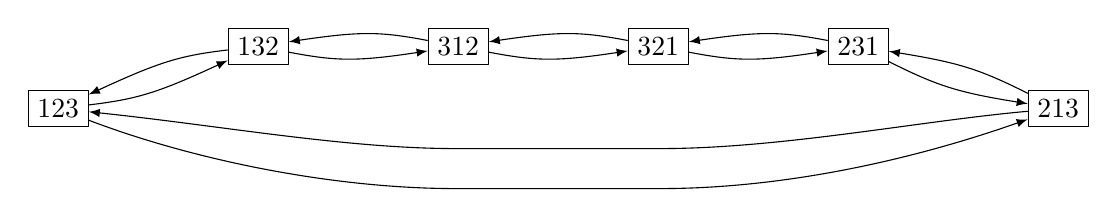
\begin{tikzpicture}[>=latex,line join=bevel,scale=0.8]
%%
\node (123) at (27.0bp,36.0bp) [draw,rectangle] {$1 \pref 2 \pref 3$};
  \node (132) at (117.0bp,64.0bp) [draw,rectangle] {$1 \pref 3 \pref 2$};
  \node (213) at (477.0bp,36.0bp) [draw,rectangle] {$2 \pref 1 \pref 3$};
  \node (312) at (207.0bp,64.0bp) [draw,rectangle] {$3 \pref 1 \pref 2$};
  \node (231) at (387.0bp,64.0bp) [draw,rectangle] {$2 \pref 3 \pref 1$};
  \node (321) at (297.0bp,64.0bp) [draw,rectangle] {$3 \pref 2 \pref 1$};
  \draw [->] (123) ..controls (62.569bp,40.26bp) and (71.703bp,43.035bp)  .. (132);
  \draw [->] (123) ..controls (88.567bp,12.545bp) and (151.46bp,0.0bp)  .. (206.0bp,0.0bp) 
.. controls (206.0bp,0.0bp) and (206.0bp,0.0bp)  .. (298.0bp,0.0bp) .. controls (347.64bp,0
.0bp) and (404.2bp,10.392bp)  .. (213);
  \draw [->] (132) ..controls (81.779bp,59.84bp) and (72.652bp,57.077bp)  .. (123);
  \draw [->] (132) ..controls (152.39bp,57.272bp) and (161.31bp,57.135bp)  .. (312);
  \draw [->] (213) ..controls (415.43bp,30.545bp) and (352.54bp,18.0bp)  .. (298.0bp,18.0bp
) .. controls (206.0bp,18.0bp) and (206.0bp,18.0bp)  .. (206.0bp,18.0bp) .. controls (156.3
6bp,18.0bp) and (99.8bp,28.392bp)  .. (123);
  \draw [->] (213) ..controls (441.87bp,53.584bp) and (432.85bp,56.597bp)  .. (231);
  \draw [->] (231) ..controls (422.48bp,46.295bp) and (431.51bp,43.289bp)  .. (213);
  \draw [->] (231) ..controls (351.95bp,70.718bp) and (343.04bp,70.864bp)  .. (321);
  \draw [->] (312) ..controls (171.95bp,70.718bp) and (163.04bp,70.864bp)  .. (132);
  \draw [->] (312) ..controls (242.39bp,57.272bp) and (251.31bp,57.135bp)  .. (321);
  \draw [->] (321) ..controls (332.39bp,57.272bp) and (341.31bp,57.135bp)  .. (231);
  \draw [->] (321) ..controls (261.95bp,70.718bp) and (253.04bp,70.864bp)  .. (312);
%
  \label{dia:DPDistance}
\end{tikzpicture}
% End of code

